\documentclass{standalone}
\usepackage{pgfplots}
\usetikzlibrary{intersections}
\usepgfplotslibrary{fillbetween}
\pgfplotsset{compat=1.7}

\begin{document}
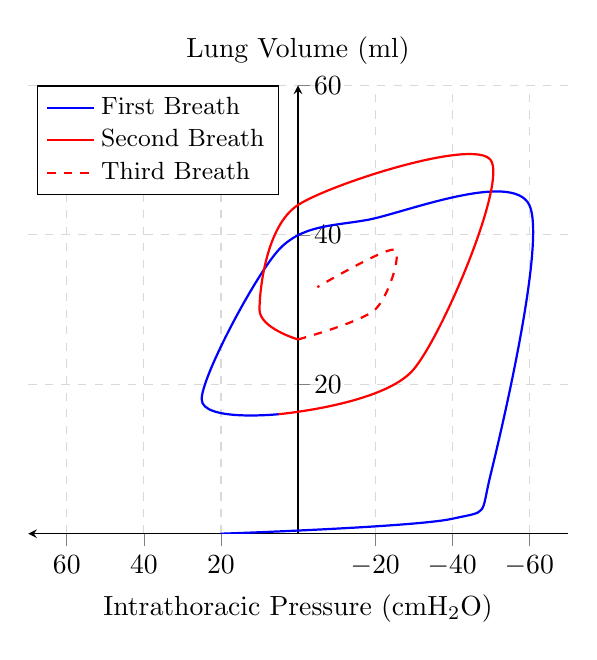
\begin{tikzpicture}


\begin{axis}[
        axis lines=middle,
        grid = major,
        grid style={dashed, gray!30},
	ymin = 0,
	ymax = 60,
	xmin = -70,
	xmax =70,
xscale=-1,
	xlabel near ticks,
every axis y label/.style={at={(current axis.north)},above=4pt},
    yticklabel style={anchor=west},
    yticklabel shift=-2pt,
        xlabel=Intrathoracic Pressure (cmH\textsubscript{2}O),
        ylabel=Lung Volume (ml),
        tick align=outside,
        enlargelimits=false,
legend style={font=\small, cells={align=left}, at={(axis cs: 5,60)}},
legend cell align={left}]

\draw[blue, thick] plot[smooth] coordinates { (axis cs: 20, 0) (axis cs: -40,2) (axis cs: -50,8) (axis cs: -60, 44)  (axis cs: -18, 42)  (axis cs: 5, 38) (axis cs: 25,18) (axis cs: 5,16)};
\draw[red, thick] plot[smooth] coordinates {(axis cs: 5,16) (axis cs: -30,22) (axis cs: -50,50) (axis cs: 0,44) (axis cs: 10,30) (axis cs: 0,26)};
\draw[red, dashed, thick] plot[smooth] coordinates {(axis cs: 0,26) (axis cs: -20,30) (axis cs: -25,38) (axis cs: -5,33)};

\addplot[blue,thick]{-1};
\addlegendentry{First Breath};
\addplot[red,thick]{-1};
\addlegendentry{Second Breath};
\addplot[red,dashed,thick]{-1};
\addlegendentry{Third Breath};

\end{axis}

\end{tikzpicture} 
\end{document}